\documentclass[8pt,a4paper,landscape]{scrartcl} 
\usepackage[left=1cm,right=1cm,top=1cm,bottom=1cm,landscape]{geometry} 
\usepackage[utf8]{inputenc} 
\usepackage[ngerman]{babel} 
\usepackage{multicol} 
\usepackage{lipsum}
\usepackage{amsmath} 
\usepackage{amsfonts} 
\usepackage{amssymb} 
\usepackage{gensymb} 
\usepackage{dsfont} 
\usepackage{calc} 
\usepackage{tabularx}
\usepackage[table]{xcolor}
\usepackage{arydshln}
\usepackage{tikz}
\usepackage{multirow}
\usetikzlibrary{calc,arrows}
%\usepackage[permil]{overpic} \usepackage{graphicx} \graphicspath{{gfx/}} 

\definecolor{Gray}{gray}{0.9}
\definecolor{LightCyan}{rgb}{0.88,1,1}


\newcolumntype{Y}{>{\centering\arraybackslash}X}
\renewcommand\tabularxcolumn[1]{m{#1}}% for vertical centering text in X column
\renewcommand{\arraystretch}{1.25}
\renewcommand{\arraycolsep}{1.25pt}
\newcommand{\tikzmark}[1]{%
	\tikz[overlay,remember picture] \node (#1) {};}


\author{Levin Baumann} 



\title{Formelsammlung Robotik} 

\begin{document} 
\setlength{\columnsep}{1cm} 
\begin{multicols*}{3}
{\LARGE\bfseries Formelsammlung Robotik }

\subsection*{Vektoren}
\renewcommand{\arraystretch}{1}
\begin{tabularx}{\columnwidth}{l|c|X}
	Skalare Multipl. & $ \lambda \cdot \vec{a}$ & 
	$\left(\begin{array}{rrr}                       \lambda \cdot a_1\\
	\lambda \cdot a_2\\
	\lambda \cdot a_3\\                 
	\end{array}\right)$\\ \hline
	Abstand P.-Urpsr. & \\
	Betrag (Norm) & $ ||\vec{a}||$ & 
	$|\vec{a}| = \sqrt{{a_1}^2 + {a_2}^2 + {a_3}^2}$\\ \hline
	Skalarprodukt & $\vec{a}\cdot\vec{b}$ & $a_1 \cdot b_1 + \ldots + a_n \cdot b_n = x$ \\ \hline
	Winkel &  & $\cos \alpha = \dfrac{\vec{a} \cdot \vec{b}}{|\vec{a}| \cdot |\vec{b}|}$ \\ \hline
\end{tabularx}

\subsection*{Matrizen}
\begin{tabularx}{\columnwidth}{r|c|X}
	Gleich & $ A = B $ & $ \left(a_{ij}\right) = \left(b_{ij}\right)$ \\ \hline
	Addition & $ C = A + B $ & $ \left(c_{ij}\right) = \left(a_{ij}\right) + \left(b_{ij}\right) $ \\ \hline
	Differenz & $ C = A - B $ &  $ \left(c_{ij}\right) = \left(a_{ij}\right) - \left(b_{ij}\right) $ \\ \hline
	Multiplikation Skalar & $ c \cdot A $ & $ cA \in R^{m \times n} $ \\ \hline
	Multiplikation Matrizen & $ A \cdot B $ & $ AB = \sum_{j} a_{ij}b_{ij} $
\end{tabularx}
%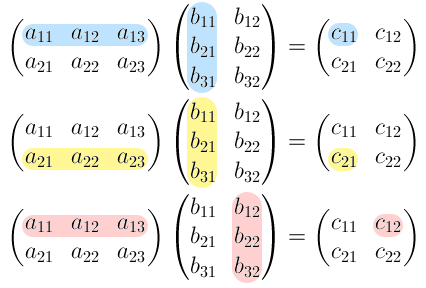
\includegraphics[width=\columnwidth]{mmultipl}

\subsubsection*{Multiplikation}

	$\left(\begin{Array}{ccc}
	\rowcolor{blue!20}
		a_{11} & a_{12} & a_{13}\\
		a_{21} & a_{22} & a_{23}\\
	\end{Array}\right)
	\cdot
	\left(\begin{Array}{>{\columncolor{blue!20}}cc}
	b_{11} & b_{12}\\
	b_{21} & b_{22}\\
	b_{31} & b_{32}
	\end{Array}\right)
	= 
	\left(\begin{Array}{cc}
	\cellcolor{blue!20} a_{11} \cdot b_{11} + a_{12} \cdot b_{21} + a_{13} \cdot b_{31} & c_{12}\\
	c_{21} & c_{22}
	\end{Array}\right)
	$\\
	$\left(\begin{Array}{ccc}
	\rowcolor{red!20}
	a_{11} & a_{12} & a_{13}\\
	a_{21} & a_{22} & a_{23}\\
	\end{Array}\right)
	\cdot
	\left(\begin{Array}{c>{\columncolor{red!20}}c}
	b_{11} & b_{12}\\
	b_{21} & b_{22}\\
	b_{31} & b_{32}
	\end{Array}\right)
	= 
	\left(\begin{Array}{cc}
	c_{11} & \cellcolor{red!20} c_{12}\\
	c_{21} & c_{22}
	\end{Array}\right)
	$\\
	$\left(\begin{Array}{ccc}
		a_{11} & a_{12} & a_{13}\\
		\rowcolor{yellow!50}
		a_{21} & a_{22} & a_{23}\\
	\end{Array}\right)
	\cdot
	\left(\begin{Array}{>{\columncolor{yellow!50}}cc}
		b_{11} & b_{12}\\
		b_{21} & b_{22}\\
		b_{31} & b_{32}
	\end{Array}\right)
	= 
	\left(\begin{Array}{cc}
		c_{11} & c_{12}\\
		\cellcolor{yellow!50} c_{21} & c_{22}
	\end{Array}\right)
	$\\

\subsection*{Rechte Hand Regel}
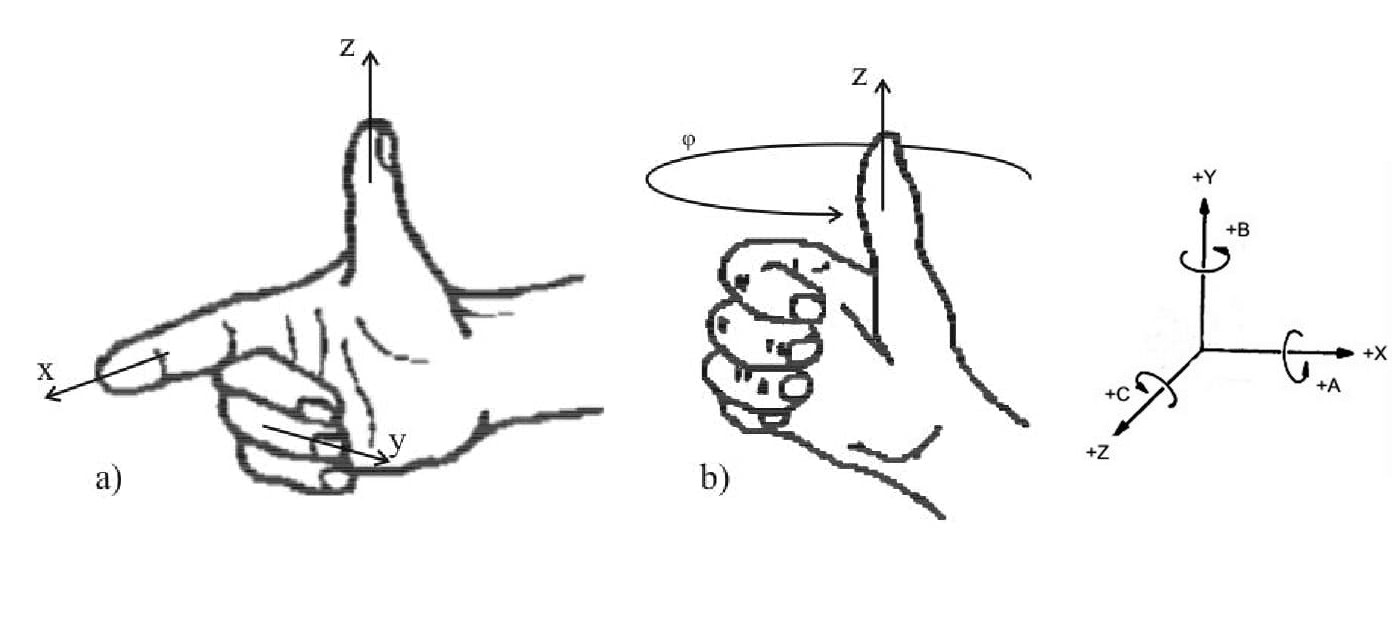
\includegraphics[width=\columnwidth]{handRotation.jpg}

\subsection*{Koordinatensysteme}
\begin{tabularx}{\columnwidth}{l|X|c}
	Objekt in 3D (OKS) & $\vec{v} = (x,y,z,\alpha,\beta,\gamma)$ & $\alpha,\beta,\gamma = $ Drehwinkel \\ \hline
	Senkrechte &  \\ 
	
\end{tabularx}

\subsection*{Rotationsmatrizen}
\begin{tabularx}{\columnwidth}{X|m{.71\columnwidth}}
	Rotation um X & $R_x(\alpha) = \left[\begin{Array}{c} x' \\ y' \\ z' \end{Array}\right]
	= \left[\begin{Array}{ccc}
		1 & 0 & 0\\
		0 & \cos\alpha & -\sin\alpha\\
		0 & \sin\alpha & \cos\alpha
	\end{Array}\right]\cdot\left[\begin{Array}{c}
		x\\
		y\\
		z
	\end{Array}\right]$\\ \hline
Rotation um Y & $R_y(\alpha) = \left[\begin{Array}{c} x' \\ y' \\ z' \end{Array}\right]
= \left[\begin{Array}{ccc}
	\cos\alpha & 0 & \sin\alpha\\
	0 & 1 & 0 \\
	-\sin\alpha & 0 & \cos\alpha
\end{Array}\right]\cdot\left[\begin{Array}{c}
	x\\
	y\\
	z
\end{Array}\right]$\\ \hline
Rotation um Z & $R_z(\alpha) = \left[\begin{Array}{c} x' \\ y' \\ z' \end{Array}\right]
= \left[\begin{Array}{ccc}
	\cos\alpha & -\sin\alpha & 0\\
	\sin\alpha & \cos\alpha & 0\\
	0 & 0 & 1
\end{Array}\right]\cdot\left[\begin{Array}{c}
	x\\
	y\\
	z
\end{Array}\right]$\\ \hline
Vormultipl. (Roll-pitch-yaw) & Rotation um die ursprüngliche (feste) Achse. Schreibweise: Letzte Drehung $\rightarrow$ 1. Drehung\\ \hline
Nachmultipl. (Euler-Winkel) & Rotation um die neuen (momentanen) Achsen. Schreibweise: 1. Drehung $\rightarrow$ Letzte Drehung\\ \hline
Homogene $4\times4$-Matrix & $\left(\begin{Array}{c|c}
	R_{3\times3} & u_{3\times1}\\ \hline
	f_{1\times3} = 0 & 1\times1
\end{Array}\right) = \left(\begin{Array}{cccc}
n_{x\downarrow z} & o_{x\downarrow z} & a_{x\downarrow z} & u_{x\downarrow z}\\
0 & 0& 0 & 1
\end{Array}\right)$\\ \hline
Invertierung 4$\times$4 &  $T^{-1} = \left(\begin{Array}{ccc:c}
	n_{x} & n_{y} & n_{z} & -n^{T}\cdot\vec{u}\\
	o_{x} & o_{y} & o_{z} & -o^{T}\cdot\vec{u}\\
	a_{x} & a_{y} & a_{z} & -a^{T}\cdot\vec{u}\\ \cdashline{1-3}
	0 & 0&0&1
\end{Array}\right)$\\ \hline
Translation um $ x,y,z $ & $ \left(\begin{Array}{cccc}
	1 & 0 & 0 & x\\
	0 & 1 & 0 & y\\
	0 & 0 & 1 & z\\
	0 & 0 & 0 & 1
\end{Array}\right) $\\ \hline
Verkettete Lagebeschr.& $ ^{BKS}H_{B}  = ^{BKS}H_{A} \cdot ^{A}H_{B}$ \hfill (H = Homo. Matr.)\\ 
\end{tabularx}

\subsection*{Quaternionen}
$$a,b,c,d \in \square \text{Quaternion } q \Rightarrow q = a + b\cdot i + c \cdot * j + d \cdot k $$
$$a \in \mathbb{R}, u = (b,c,d)^T \in \mathbb{I}$$
$$q = (a,b,c,d)^T \text{ bzw. } q=(a,u)^T$$
\begin{alignat*}{3}
	i^2 &= j^2 &= k^2 &= ijk = -1\\
	ij &= -ji &= k\\
	jk &= -kj &= i\\
	ki &= -ik &= j
\end{alignat*}

\begin{tabularx}{\columnwidth}{m{.15\columnwidth}|>{\raggedright\arraybackslash}X}
	Gegeben & $ q = (a_q, u_q), r=(a_r, u_r) $\\ \hline
	Addition & $ q + r = (a_q + a_r, u_q + u_r) $\\ \hline
	Skalar & $ q \cdot r = a_qa_r + <u_q, u_r> = a_qa_r + b_qb_r + c_qc_r +d_qd_r $\\ \hline
	quatern. Multipl. & $  q*r = \newline (a_q+i\cdot b_q + j\cdot c_q + k\cdot d_q)\cdot (a_r + i\cdot b_r + j\cdot c_r + k\cdot d_r) $\\ \hline
	konjugiert & $ q^{*} = (a_q, -u_r) $\\ \hline
	Norm & $ |q| = \sqrt{qq^{*}} = \sqrt{q^{*}q} = \sqrt{a^2+b^2+c^2+d^2} $\\ \hline
	inverses Element & $ q^{-1} = \frac{q^{*}}{|q|^2}$
\end{tabularx}

\subsubsection*{Rotation mit Quaternionen}
\begin{tabularx}{\columnwidth}{l|X}
	Vektor als Quaternion & $ p = (x,y,z)^T \Leftrightarrow q_p = (0, p)^T $\\ \hline
	Skalar als Quaternion & $ s \Leftrightarrow q_s = (s, 0, 0, 0)^T $\\ \hline
	Einheitsquaternion & $ |q| = 1 $\\ \hline
	Rotation um $ \theta $, Achse $ u $ & $ q_r = (\cos(\frac{\theta}{2}), u\cdot\sin(\frac{\theta}{2})) $\\ \hline
	Rotation Punkt $ p $ & $ q_{p'} = q_rq_pq_r^{*} = q_rq_pq_r^{-1} $
\end{tabularx}

\subsection*{Sinus}
\begin{tabularx}{\columnwidth}{r|c|c|c|c|c|c|c|c|c}
	$ a° $ & $ 0° $ & $ 30° $ & $ 45° $ & $ 60° $ & $ 90° $ & $ 120° $ & $ 135° $ & $ 150° $ & $ 180° $ \\ \hline
	$ \sin a$& $ 0 $& $ \frac{1}{2} $& $ \frac{\sqrt{2}}{2} $& $ \frac{\sqrt{3}}{2} $& $ 1 $& $ \frac{\sqrt{3}}{2} $& $ \frac{\sqrt{2}}{2} $& $ \frac{1}{2} $& $ 0 $\\ \hline
	$ \cos a$& $ 1 $& $ \frac{\sqrt{3}}{2} $& $ \frac{\sqrt{2}}{2} $& $ \frac{1}{2} $& $ 0 $& $ -\frac{1}{2} $& $ -\frac{\sqrt{2}}{2} $& $ -\frac{\sqrt{3}}{2} $& $ -1 $
\end{tabularx}

\subsubsection*{Trigonometrie}
$$ \sin(\alpha + \beta) = \sin\alpha \cdot \cos\beta + \sin\beta \cdot \cos\alpha $$
$$ \cos(\alpha + \beta) = \cos\alpha \cdot \cos\beta - \sin\alpha \cdot \sin\beta $$

\end{multicols*}
\end{document}